 \documentclass[12 pt]{book}
\usepackage{amsmath}
\usepackage{amsthm}
\usepackage[paperwidth=5 in,paperheight=5 in,left=9 mm, right=9 mm, top=15 mm, bottom=18.5 mm]{geometry}
\usepackage{graphics}
\usepackage{fontawesome}
\usepackage{enumitem}
\usepackage{marvosym}
\newcommand{\myitem}{\refstepcounter{enumi}\item[$^\star$\theenumi.]}
\newcommand{\mmyitem}{\refstepcounter{enumi}\item[$^{\star \star}$\theenumi.]}
\setcounter{page}{01}

\usepackage[utf8]{inputenc}
\usepackage{xcolor}
\setlength{\arrayrulewidth}{0.1 mm}
%BLUE%
%\definecolor{Mycolor2}{HTML}{3D9BE9}
\definecolor{Mycolor2}{HTML}{33cccc}
%\definecolor{Mycolor2}{HTML}{000000}

%%----HEADER &&& FOOTER----%%

\usepackage{fancyhdr}


\pagestyle{fancy}
\fancyhf{}
\setlength{\headheight}{8 mm}
%\fancyhead[CE,CO]{ \Times\Large{\textbf{\textls*[100]{\textcolor{tomato}{\textit{Illustration}}}}}}

\fancyhead[CE,CO]{\Large{\textbf{\textls*[250]{\textcolor{tomato}{SOLVE ME! \\[-5 mm]{\Large{\textbf{\textls*[5000]{\textcolor{black}{\scalebox{.42}{ROTATION}}}}}}     }}}}}

\fancyfoot[RE,RO]{\large{\textbf{\textls*[10]{\textcolor{tomato}{\Times\textit{Solution~\boldmath$\rightarrow$}}}}}}

\renewcommand{\headrulewidth}{0 mm}
\renewcommand{\footrulewidth}{0 mm}


\DeclareMathOperator{\Ln}{ln}

%%----FONT &&& MATHS_FONT----%%

\usepackage{amssymb}
\usepackage{upgreek,xspace}
\newcommand*{\rom}[1]{\expandafter\@\romannumeral #1}


\usepackage[utopia]{mathdesign}
\renewcommand{\familydefault}{\sfdefault}
\usepackage[scaled=1]{helvet}
\newcommand*\Times{\fontfamily{ptm}\selectfont}

%%%------PACAKAGES------%%%

\usepackage[letterspace=120]{microtype}
\usepackage{enumitem}
\usepackage{multicol}
\usepackage{pgfplots}
\pgfplotsset{width=8cm,compat=1.16}
\usepackage{tikz}
\usepgfplotslibrary{fillbetween}
\usetikzlibrary{quotes,angles,patterns,through,calc}
\usepgflibrary{arrows.meta}
\usetikzlibrary{decorations.pathmorphing}
\usetikzlibrary{decorations.markings}
\usetikzlibrary{arrows.meta,bending}
\usepackage{rotating}
\usepackage{tikz-3dplot}
\usepackage[american voltages, american currents,siunitx]{circuitikz}
\usepackage{circuitikz}
\usetikzlibrary{fit,positioning}
\usetikzlibrary{optics}
\usetikzlibrary{intersections}
\usetikzlibrary{decorations.pathreplacing}
\usepackage{setspace}
\setstretch{1.1}


\usepackage{vwcol}[widths={0.25,0.75}]


\usepackage{color}
\usepackage[autostyle]{csquotes}


\usepackage{xcolor}
\definecolor{Mycolor2}{HTML}{33cccc}
\definecolor{One}{HTML}{336666}
\definecolor{Two}{HTML}{666666}
\definecolor{Three}{HTML}{cc6699}


%  black--brown--black %
\definecolor{Four}{HTML}{000000}
\definecolor{Five}{HTML}{330000}
\definecolor{Six}{HTML}{000000}

\definecolor{Seven}{HTML}{ff6666}
\definecolor{Eight}{HTML}{330066}
\definecolor{Nine}{HTML}{cc3333}
\definecolor{tomato}{HTML}{FF6347}
\definecolor{darkblue}{HTML}{2c3e50}
\definecolor{blackm}{HTML}{363636}
\definecolor{pink}{HTML}{ff6666}


\newcommand{\nm}{\begin{minipage}[c]{0.1\linewidth}
{\Huge{\textcolor{tomato}{\textbf{5. }}}}
\end{minipage}}

\newcommand{\sm}{\begin{minipage}[c]{0.1\linewidth}
{\Huge{\textcolor{tomato}{\textbf{ }}}}
\end{minipage}}

\newcommand{\AxisRotator}[1][rotate=0]{%
    \tikz [x=0.25cm,y=0.60cm,line width=.2ex,-stealth,#1] \draw (0,0) arc (-120:120:1 and 1);%
}

\newcommand{\vl}{{{\textcolor{tomato}{\textbf{\vrule width 2.25 pt{}}}}}}

\newenvironment{question}
{	
	\nm  \vl \,
	\begin{minipage}[l]{0.86\linewidth}
	\begin{itshape}
	\normalsize\Times\textit{}
}
{
	\end{itshape}
	\end{minipage}
}


\newenvironment{options}
{	
	\sm ~
	\begin{minipage}[l]{0.86\linewidth}
	\begin{multicols}{2}
	\begin{enumerate}[label={(\roman*)}, itemsep=4 mm]
	\normalsize{}
}
{
	\end{enumerate}
	\end{multicols}
	\end{minipage}
}


\newenvironment{v-options}
{	
	\sm ~
	\begin{minipage}[l]{0.86\linewidth}
	\begin{enumerate}[label={(\roman*)}, itemsep=4 mm]
	\normalsize{}
}
{
	\end{enumerate}
	\end{minipage}
}



\newenvironment{definition}
{
	\begin{center}
	\begin{itshape}
	\normalsize\Times\textit{}
}
{
	\end{itshape}
	\end{center}
}


\newenvironment{note}
{
	\begin{center}
	\begin{itshape}
	\normalsize\Times\textit{}
}
{
	\end{itshape}
	\end{center}
}

\newenvironment{q-options}
{	
	\sm ~
	\begin{minipage}[l]{0.86\linewidth}
	\begin{note}
	\begin{enumerate}[label={(\roman*)}, itemsep=1 mm]
	\normalsize{}
}
{
	\end{enumerate}
	\end{note}
	\end{minipage}
}



\newcommand{\physics}{\normalsize{\textcolor{tomato}{\textls*[100]{{\hspace*{75 mm} @10xphysics}}}}}

\newcommand{\solution}{\centering\Large\Times\textbf{\textcolor{tomato}{\textls*[100]{ \textit{\\[-20 mm]Solution}}} }}

\begin{document}


\nopagecolor
%\boldmath
\color{black!100}
%\pagecolor{black!95}
\setlength{\parindent}{0pt}
\large

%%%%   PROBLEM-02  %%%%%

\begin{question}
A rod of mass $m$ and length $l$ makes angle $\theta$ with the floor is being pulled with a constant velocity $v_0$ as shown in figure. Find the angular velocity of the rod when $\theta$ becomes $37^\circ$.\\
\end{question}

{\physics}



\begin{center}
\begin{tikzpicture}[use optics,very thick,decoration={
    markings,
    mark=at position 0.3 with {\arrow{Stealth}}},every node/.style={scale=0.85},yscale=0.65]
\node[thick,mirror,rotate=-90,scale=2.75,mirror decoration separation=0.08,mirror decoration amplitude=0.12] at (2.33,0) {};
\node[thick,mirror,rotate=-180,scale=1.5,mirror decoration separation=0.08,mirror decoration amplitude=0.12] at (0,2) {};
\draw[line width=5,line cap=round] (0.08,3) coordinate (b)--([turn]-135:4) coordinate (a);
\coordinate (c) at (0,-0.5);
\pic [thick,draw=black,"$\theta$", angle eccentricity=1.45,angle radius=0.6cm] {angle = b--a--c};
\draw [-Stealth] (3,0.25) -- (4,0.25)node[right]{$v_0$};
\end{tikzpicture}
\end{center}

\vspace*{5 mm}

\begin{note}
Comment down your answer.
\end{note}

\pagebreak


\pagestyle{empty}

\begin{center}
{\solution}
\end{center}


\begin{center}
\begin{tikzpicture}[use optics,thick,decoration={
    markings,
    mark=at position 0.3 with {\arrow{Stealth}}},every node/.style={scale=0.85},scale=1.5]
%\node[thick,mirror,rotate=-90,scale=2.75,mirror decoration separation=0.08,mirror decoration amplitude=0.12] at (2.33,0) {};
%\node[thick,mirror,rotate=-180,scale=1.5,mirror decoration separation=0.08,mirror decoration amplitude=0.12] at (0,2) {};
\draw[line width=5,line cap=round] (0,3) coordinate (b)--([turn]-135:4) coordinate (a);
\coordinate (c) at (0,0);
\pic [thick,draw=black,"$\theta$", angle eccentricity=1.5,angle radius=0.65cm] {angle = b--a--c};
\draw [-Stealth] (a) -- ++(1.25,0) coordinate (d) node[right]{$v_0$};
\draw [-Stealth] (a) -- ++(1,-1) coordinate (e) node[right]{$v_0 \cos\theta$};
\pic [thick,draw=black,"$\theta$", angle eccentricity=1.5,angle radius=0.65cm] {angle = e--a--d};
\draw [-Stealth] (a) -- ++(1.25,1.25) coordinate (e) node[right]{$v_0 \sin\theta$};
\draw[dashed] (a)-- ++(-1.25,0);
\draw [-Stealth] (b) -- ++(0,-1.25) coordinate (f) node[right]{$v'$};
\draw [-Stealth] (b) -- ++(-1.25,-1.25) coordinate (g) node[below]{$v'\cos\theta$};
\pic [thick,draw=black,"$\theta$", angle eccentricity=1.5,angle radius=0.65cm] {angle = g--b--f};
\draw [-Stealth,tomato] (b) -- ++(1,-1) coordinate (g) node[right]{$v'\sin\theta$};
\node at  (2*cos 43, 1.53)[tomato] {$\bullet$};
\node at  (2*cos 43, 1.5)[tomato] {\AxisRotator[rotate=200]};
\end{tikzpicture}
\end{center}

{\physics}



\pagebreak

\begin{note}
Velocity along the rod will remain same for both ends.
\begin{align*}
v_0 \cos\theta &= v'\sin\theta \\
v' &= v_0 \cot\theta \\
v' &= v_0 \cot 37^\circ \\
	&= \dfrac{4v_0}{3} \\[15 mm]
\textit{angular velocity} &= \dfrac{\textit{relative perpendicular velocity}}{\textit{length of the rod}} \\[7 mm]
\omega &= \dfrac{v_0 \sin\theta + v' \cos\theta}{l}
\end{align*}


\pagebreak

\begin{align*}
\omega &= \dfrac{v_0 \sin 37^\circ + v' \cos 37^\circ}{l} \\[2 mm]
			&= \dfrac{ \dfrac{3v_0}{5} +  \dfrac{4v'}{5}}{l} \\[2 mm]
			&= \dfrac{ \dfrac{3v_0}{5} +  \dfrac{4}{5} \times \dfrac{4v_0}{3} }{l} \\[2 mm]
			&= \dfrac{5v_0}{3l} \\[2 mm]
\end{align*}

\end{note}

{\physics}

\pagebreak

\end{document}